% Harus dimuat terlebih dahulu, digunakan agar file PDF memiliki format karakter yang benar.
% Untuk informasi lebih lanjut, lihat https://ctan.org/pkg/cmap.
\RequirePackage{cmap}

% Format dokumen sebagai paper konferensi menggunakan aturan IEEEtran terbaru (v1.8b).
% Untuk informasi lebih lanjut, lihat http://www.michaelshell.org/tex/ieeetran/.
\documentclass[a4paper, conference]{IEEEtran}
\usepackage[left=1.57cm,right=1.57cm,top=0.95cm,bottom=2.54cm]{geometry}

% Format encoding font dan input menjadi 8-bit UTF-8.
\usepackage[T1]{fontenc}
\usepackage[utf8]{inputenc}

% Format bahasa menjadi bahasa german dan inggris.
%\usepackage[indonesian]{babel}

% Digunakan untuk tujuan demonstrasi.
\usepackage{mwe}

% Digunakan untuk menampilkan font dengan style yang lebih baik.
\usepackage[zerostyle=b,scaled=.75]{newtxtt}

% Digunakan untuk menampilkan tabel dengan style yang lebih baik.
\usepackage{booktabs}

% Digunakan untuk menampilkan gambar pada dokumen.
\usepackage{graphicx}

% Digunakan untuk menampilkan potongan kode.
\usepackage{listings}
\lstset{
  basicstyle=\ttfamily,
  columns=fixed,
  basewidth=.5em,
  xleftmargin=0.5cm,
  captionpos=b
}

% Digunakan agar backticks (`) dapat dirender pada PDF.
% Untuk informasi lebih lanjut, lihat https://tex.stackexchange.com/a/341057/9075.
\usepackage{upquote}

% Digunakan untuk menyeimbangkan bagian akhir dokumen dengan dua kolom.
\usepackage{balance}

% Digunakan untuk menampilkan pustaka.
\usepackage[square,comma,numbers,sort&compress]{natbib}

% Mengubah format ukuran teks pada natbib.
\renewcommand{\bibfont}{\normalfont\footnotesize}

% Menambah nama penulis ketika menggunakan perintah \citet.
% Untuk informasi lebih lanjut, lihat https://tex.stackexchange.com/a/76075/9075.
\usepackage{etoolbox}
\makeatletter
\patchcmd{\NAT@test}{\else \NAT@nm}{\else \NAT@hyper@{\NAT@nm}}{}{}
\makeatother

% Digunakan untuk menambah hyperlink pada referensi.
\usepackage{hyperref}

% Menonaktifkan warna dan bookmark pada hyperref.
\hypersetup{hidelinks,
  colorlinks=true,
  allcolors=black,
  pdfstartview=Fit,
  breaklinks=true
}

\usepackage{tabularx}
\usepackage{amsmath}
\usepackage{multirow}

% Digunakan untuk membenarkan hyperref pada gambar.
\usepackage[all]{hypcap}

% Digunakan untuk menampilkan beberapa gambar
\usepackage[caption=false,font=footnotesize]{subfig}

\usepackage{stfloats}

% Tambahkan format tanda hubung yang benar di sini
\hyphenation{}

\begin{document}

% Ubah kalimat berikut sesuai dengan judul penelitian.
\title{Kalkulasi Energi pada Roket Luar Angkasa \\ Berbasis \emph{Anti-Gravitasi}}

% Ubah kalimat-kalimat berikut sesuai dengan nama, institusi, alamat dan kontak penulis.
\author{
  \IEEEauthorblockN{Elon Reeve Musk}
  \IEEEauthorblockA{Departemen Teknik Dirgantara\\
    Fakultas Teknologi Dirgantara\\
    Institut Teknologi Sepuluh Nopember\\
    Surabaya, Indonesia 60111\\
    elon.musk@mhs.its.ac.id}

  \and
  \IEEEauthorblockN{Nikola Tesla}
  \IEEEauthorblockA{Departemen Teknik Dirgantara\\
    Fakultas Teknologi Dirgantara\\
    Institut Teknologi Sepuluh Nopember\\
    Surabaya, Indonesia 60111\\
    \url{https://nikolatesla.me}}

  \and
  \IEEEauthorblockN{Wernher von Braun}
  \IEEEauthorblockA{Departemen Teknik Dirgantara\\
    Fakultas Teknologi Dirgantara\\
    Institut Teknologi Sepuluh Nopember\\
    Surabaya, Indonesia 60111\\
    von.braun@td.its.ac.id}
}

% Digunakan untuk menampilkan judul dan deskripsi penulis.
\maketitle

% Mengubah keterangan `Abstract` ke bahasa indonesia.
% Hapus bagian ini untuk mengembalikan ke format awal.
\renewcommand\abstractname{Abstrak}

\begin{abstract}

  % Ubah paragraf berikut sesuai dengan abstrak dari penelitian.
  Fake news or called hoax, is one of the things that still plaguing Indonesia. Even more so, with the rise of the social media, a fake news can spread wider and faster than ever before. Worse, Indonesian people have quite a high tendencies to share fake news. That is why, we are in a dire need of a method to detect fake news. This research is using BERT to automatically classifiy whether a news is a hoax or not. From a raw text, we applied a tokenization process before inputting the text to the BERT. Next, the pooled output of the BERT is being used as the input for Linear Regression, a tested-and-true method for classifying task. The output of the Linear Regression is then being used as a way to determine whether a news is a hoax or not. The purpose of this research is to create a machine learning model to help the people to determine whether a text is a fake news or not. The result of this research is a model to classify a hoax text with 89\% in accuracy.

\end{abstract}

% Mengubah keterangan `Index terms` ke bahasa indonesia.
% Hapus bagian ini untuk mengembalikan ke format awal.
\renewcommand\IEEEkeywordsname{Kata kunci}

\begin{IEEEkeywords}

  % Ubah kata-kata berikut sesuai dengan kata kunci dari penelitian.
  BERT, Hoax, Fake News Classification, Linear Regression

\end{IEEEkeywords}


% Ubah bagian berikut sesuai dengan konten-konten yang akan dimasukkan pada dokumen
% Ubah judul dan label berikut sesuai dengan yang diinginkan.
\section{Pendahuluan}
\label{sec:pendahuluan}

% Ubah paragraf-paragraf pada bagian ini sesuai dengan yang diinginkan.

Pesatnya perkembangan roket yang merupakan \lipsum[2-4]

Pembahasan pada paper ini dimulai dengan presentasi mengenai penelitian lain (Bagian \ref{sec:penelitianterkait}).
Kemudian dilanjutkan dengan penjelasan mengenai arsitektur dari sistem yang dibuat (Bagian \ref{sec:arsitektur}).
Berdasarkan hal tersebut, kami menunjukkan lorem ipsum (Bagian \ref{sec:loremipsum}).
Terakhir, didapatkan kesimpulan dari penelitian yang telah dilakukan (Bagian \ref{sec:kesimpulan}).

%% Ubah judul dan label berikut sesuai dengan yang diinginkan.
\section{Penelitian Terkait}
\label{sec:penelitianterkait}

% Ubah paragraf-paragraf pada bagian ini sesuai dengan yang diinginkan.

Beberapa penelitian lain pernah dilakukan seperti yang dirumuskan oleh \citet{newton1687} bahwa \lipsum[5]
Hasil tersebut kemudian menjadi persamaan \ref{eq:hukumpertama}.

% Contoh pembuatan persamaan ilmiah.
\begin{equation}
  \label{eq:hukumpertama}
  \sum \mathbf{F} = 0\; \Leftrightarrow\; \frac{\mathrm{d} \mathbf{v} }{\mathrm{d}t} = 0.
\end{equation}

\lipsum[6-7]

% Ubah judul dan label berikut sesuai dengan yang diinginkan.
\section{Design and Implementation}
\label{sec:designandimplementation}

% Ubah paragraf-paragraf pada bagian ini sesuai dengan yang diinginkan.
This research is explaining about the implementation of one of the branch of deep learning studies with the aim to automatically detect Indonesian hoax news by leveraging BERT method. This detection method is trained by using a combination of dataset from \url{https://data.mendeley.com/datasets/p3hfgr5j3m/1} and dataset that we made ourself for this paper alone by using web crawling technology. Picture \ref{fig:metodologi} is the outline of this research in a nutshell.

\begin{figure} [h!]
    \centering
    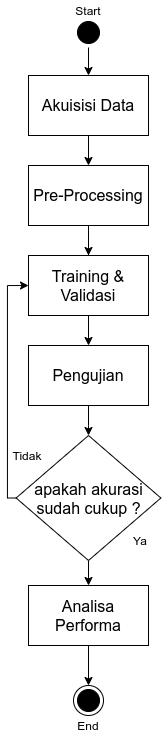
\includegraphics[width=0.3\columnwidth]{gambar/metodologi_vertical.png}
    \caption{This research method in a nutshell.}
    \label{fig:metodologi}
\end{figure}

\subsection{Material and Tools Specification}

The dataset that is being used in this research is a dataset originated from \url{https://data.mendeley.com/datasets/p3hfgr5j3m/1} coupled with our own made dataset in which we have create it using web crawling technology. Both of these dataset combined, is resulting in total of 1621 data with the exact details can be seen at table \ref{tab:dataset}. Meanwhile, table \ref{tab:dataset_mendeley} is the starting point of our dataset which we gotten from \url{https://data.mendeley.com/datasets/p3hfgr5j3m/1} alone.

Each of these dataset is containing the content of the news along with its label which can be either "Valid" or "Hoaks". We took the news from accredited and verified news sources for the valid news, while on the other side, we took all of the hoax news mostly from \url{https://turnbackhoax.id}, a website that contains the list of user reported hoax news from many sources.

\begin{table}[h]
    \caption{Total of news from \url{data.mendeley.com}}
    \label{tab:dataset_mendeley}
    \centering
    \begin{tabular}{ | l | l | }
        \hline
        \textbf{Label} & \textbf{Total Data} \\ \hline
        \textit{Hoaks} & 228                 \\ \hline
        \textit{Valid} & 372                 \\ \hline
        \textbf{Total} & \textbf{600}        \\ \hline
    \end{tabular}
\end{table}

\begin{table}[h]
    \caption{Total of training dataset}
    \label{tab:dataset}
    \centering
    \begin{tabular}{ | l | l | }
        \hline
        \textbf{Label} & \textbf{Total Data} \\ \hline
        \textit{Hoaks} & 885                 \\ \hline
        \textit{Valid} & 736                 \\ \hline
        \textbf{Total} & \textbf{1621}       \\ \hline
    \end{tabular}
\end{table}


\begin{table}[h]
    \caption{Dataset Sample}
    \label{tab:contoh_dataset}
    \centering
    \begin{tabular}{ | p{.8\linewidth} | l | }
        \hline
        \textbf{news}                                                                                                                                                                                                                     & \textbf{tagging} \\ \hline
        Wakil Gubernur DKI Jakarta Sandiaga Uno menargetkan pengerjaan tahap awal Stadion BMW dilakukan pada Oktober. Stadion ini diperuntukkan bagi klub Persija....                                                                     & Valid            \\ \hline
        "Komisi II bersama KPU dan Bawaslu masih membahas ketentuan wajib cuti bagi petahana presiden yang maju Pilpres 2019. Mekanisme pengambilan.....                                                                                  & Valid            \\ \hline
        Jaksa penuntut Ulumum (JPU) pada Komisi Pemberantasan Korupsi (KPK) mencecar Pejabat Pembuat Komitmen (PPK) reguler pada Direktorat Perlindungan Sosial Korban Bencana Sosial Kemensos Victorious Saut Hamonangan Siahaan soal... & Valid            \\ \hline
        “Halo Kak! Aku Winda Dari Team Giveaway BAIM WONG Anda Memenangkan Hadiah Uang 100Jt dari kami info klik: https://wa.me/+6285796306857”                                                                                           & Hoax             \\ \hline
        “Apa yang terjadi dengan hewan dalam penelitian?   Teknologi ini telah dicoba pada hewan, dan pada hewan penelitian yang dilakukan, semua hewan mati , tidak langsung dari suntikan...                                            & Hoax             \\ \hline
        “Kadrun istilah dr PKI alias KOMUNIS ditujukan buat islam. Kl mau jd komunis pake aja istilah kadrun buat umat islam. Auto lsg Komunis”                                                                                           & Hoax             \\ \hline
    \end{tabular}
\end{table}

\subsection{Data Acquisition}

Because the dataset that we get from \url{https://data.mendeley.com/datasets/p3hfgr5j3m/1} feel severely lacking for our purpose because it only consist of 600 data, and because there are no web crawling which outputting its result into a convenient CSV file from Indonesian news sites, we took on our hand a task to create a webcrawling program to take news content from many Indonesian news sites, those sites included but not limited to \url{liputan6.com}, \url{detik.com}, \url{tempo.com} and others. As all of those sites is rightfully accredited and verified by the government, it is used for our valid news dataset. Our hoax news site however, only has one source from \url{turnbackhoax.id}, this is mainly because said site has quite an active forum behind it in which lots of people can report their finding of hoax text, seen and checked by lots of other people, before lastly, will be uploaded to the \url{turnbackhoax.id} site. But, the biggest factor in choosing that site compare to others is mainly because \url{turnbackhoax.id} wrote the original hoaxes text in their website, this coupled with the fact that their website has some kind of structure into it has shorten our task significantly. For this research, the webcrawling process has took news from varied dates, ranging from April 2018 as the oldest to April 2021.

\begin{figure} [h!]
    \centering
    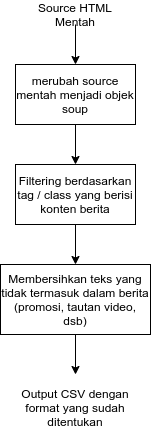
\includegraphics[width=0.35\linewidth]{gambar/webcrawl_long.png}
    \caption{Garis besar alur program \textit{web crawl}.}
    \label{fig:webcrawl_method}
\end{figure}

Picture \ref{fig:webcrawl_method} is the outline flow of the webcrawling program. Starting with inputting raw HTML code into the program, changing said code into an easier-to-process objects, get the news text and do some post-cleaning on the text, lastly, create a .CSV file to store all of the obtained news text with the appropriate format.

\begin{lstlisting}[
    language=HTML, 
    caption={Penggalan Kode Sumber HTML \url{detik.com}.},
    label={lst:source_detik}
]

...
<div class="detail__body itp_bodycontent_wrapper">
<div class="detail__body-text itp_bodycontent">

<strong>Jakarta</strong> - Koalisi <a href="https://
detik.com/tag/jokowi" target="_blank">Jokowi</a> 
sedang menyusun visi-misi jagoannya. Setelah 
menerima masukan dari <a href="https://detik.com/
tag/muhammadiyah" target="_blank"> Muhammadiyah</a>,
 ... 
Dan kita pun membuka diri untuk menerima 
masukan untuk penyempurnaan," imbuhnya.<br><br><!--
s:parallaxindetail--><div class="clearfix"></div><style>
...

\end{lstlisting}

Firstly, we need to determine tag or class of the HTML code for our first filter. If we look into listing \ref{lst:source_detik} as a reference, we can see \texttt{detail\_\_body\-text} class is the one that containing our desired news text. We filtered that class by inputting the class name into the appropriate parameter.

More often than not, our filtering result will contain some garbage or unrelated text resulting in the need to refine it further by post-clean it after the filter process. Usually, those text is writer or editorial notes, ad, or related news links which we don't need at all.

Finally, the last step is outputting all of the acquired news text as a .CSV file. There are no particular reason on the article of why we chose CSV file format compared to other famous file format aside from the CSV file format is easier to use in our training program and because it is an open-format that can be opened and edited if need be, by nearly any spreadsheet program.

As the general interface and improving user experience for our webcrawling software, we use a .json format file to configure what news sources that we want to get, how much is it, and when is it. All of those configuration will be processed by the program and the program will take the news in accordance with said configuration.

\subsection{Preprocessing}

\begin{figure}[h!]
    \begin{center}
        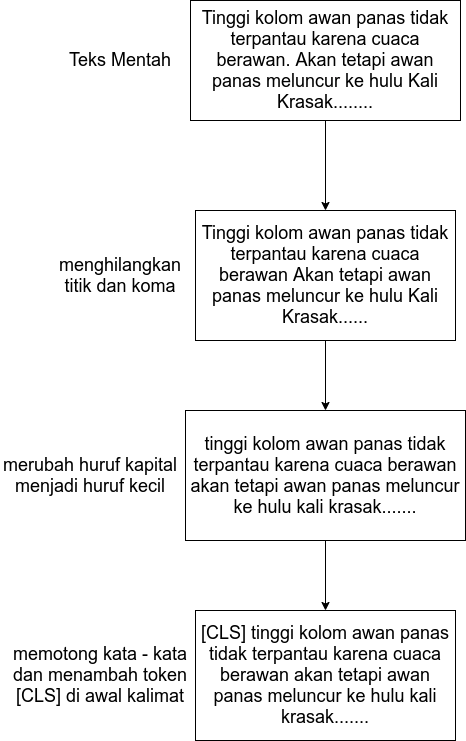
\includegraphics[width= .7\linewidth]{gambar/preprocess_long.png}
        \caption{Preprocessing Method}
        \label{fig: metodologi_preprocessing}
    \end{center}
\end{figure}

In this particular process, data need to be prepared first thing before being processed into BERT. This data preprocessing method is consisted of removing any punctuation in the text, change all of the capital letter into its lower letter and truncate any texs that is longer than the capacitites of word that BERT could process at once that is at 512 words or token. There are a few options on how to truncate the text, for example we can take the first 512 words and delete the rest, we can take the last 512 words, or we can combine from both the start of the text and the end portion of the text with some ratio. Last step of this preprocessing is to add a special \texttt{[CLS]} token. Picture \ref{fig: metodologi_preprocessing} will explain the same thing but with a better clarity.

Other than that, we will also divide the dataset into 3 portionss with details stated below :

\begin{itemize}
    \item 70\% Training, 10\% Validation, 20\% Test
\end{itemize}

\begin{enumerate}
    \item Training

          This set is used with BERT as an input when it is in its training phase so we can get an optimized model for our task.

    \item Validation

          This set is used right after BERT finished its training phase. Used to determined whether our created model has appropriate weight for our task or if our model still need to be trained again. This portion is also used to determine whether our model is overfitting or underfitting which is a bad thing.

    \item Test

          This set is used as an accuracy test after both the validation and the training phase is finished. The resulting accuracy of this set is the one that we consider as our result.

\end{enumerate}

To make it clearer, check table \ref{tab:dataset_section}. We can see based on this table that the divition of the dataset is already appropriate.

\begin{table}[h]
    \caption{Dataset Portioning Details}
    \label{tab:dataset_section}
    \centering
    \begin{tabular}{ | l | l | l | l | }
        \hline
        \textbf{Bagian}                      & \textbf{Hoaks} & \textbf{Valid} & \textbf{Total Data} \\ \hline
        \textit{Training}                    & 647            & 519            & 1166                \\ \hline
        \textit{Validasi}                    & 85             & 78             & 163                 \\ \hline
        \textit{Pegujian}                    & 153            & 139            & 292                 \\ \hline
        \multicolumn{3}{|l|}{\textbf{Total}} & \textbf{1621}                                         \\ \hline
    \end{tabular}
\end{table}

\subsection{The Architecture of BERT}

BERT is one of the latest machine learning implementation at this time especially for Natural Language Processing (NLP) task. It is based on the Transformer implementation that is based on a previous research by Vaswani et al. \cite{attention_is_all_you_need}. BERT has successfully achieved a higher accuracy than ever before in understanding the context of a raw text if compared to other transformer implementation.

One of the distinct feature of BERT is in the way it is pre-trained. There are 2 steps for pretraining BERT. The first is by doing a Masked Language Model (MLM) in which BERT will be given masked text A and some words B that can be the correct word for the masked text or not as an input, and it will need to predict whether the word B is the correct word for the masked part in text A. This way, BERT will be able to "learn" the relationship between words. The next steps for pretraining BERT is to do some Next Sentence Prediction (NSP) task. The inputted text of this task is 2 sentence, sentence A and sentence B and BERT task is to predict whether these 2 sentences will form a complete paragraph or not. By doing NSP tasks, BERT should be able to get the relationship between sentences easier.

\begin{figure*}[h!]
    \begin{center}
        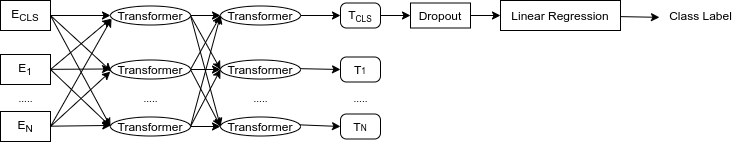
\includegraphics[width= 0.9\textwidth]{gambar/bert_arch.png}
        \caption{The Architecture of BERT in this research}
        \label{fig: bert_arch}
    \end{center}
\end{figure*}

In this research, we decided to use fine-tuning approach, what this mean is that we use a pre-trained BERT model rather than create our own BERT model from scratch, however, we still need to connect the last layer of BERT into a classification layer. In this case, we chose Linear Reggression as the classification layer. For greater detail, figure \ref{fig: bert_arch} is the architecture of BERT that will be used throughout this research.

\subsection{Training and Validation}

\begin{figure}[h!]
    \begin{center}
        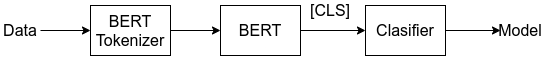
\includegraphics[width= 0.9\linewidth]{gambar/training.png}
        \caption{Training Method}
        \label{fig: metodologi_training}
    \end{center}
\end{figure}

At this stage, the raw text that will be inputted into BERT has already going through its preprocessing phase and is now going into a process called Tokenizer. Tokenizer is a process to change words in a text into token according to its word embedding that is already obtained beforehand when BERT is still in its pretraining phase. Only after all of these process has done, BERT will start its training phase based on the tokenized and preprocessed data.

Not all of the output of the BERT is being used in this particular research, we only need the content of the \texttt{[CLS]} token that is filled with the pooled output of all the other tokens and layers. The content of the \texttt{[CLS]} token is then inputted into Linear Regresson method. This method is choosen as it is easy enough while still retain quite good accuracy. Figure \ref{fig: metodologi_training} is the training method in a nutshell.

There are also some parameters that we can adjust only in this stage, namely batch, learning rate, and epoch. Batch is a parameter to adjust how much data is being processed at once per iteration, mind you that there are usually a few iteration per epoch. By adjusting the batch values, the higher it is, the faster the training process is but at the cost of the memory usage. Thanks to BERT method having quite a large number of layers (718 layers, in general) it can be considered quite heavy, hence we are set the batch value at 10.

Epoch is how much training and validation will take place before the training phase is considered as final. This parameter is one of the most important parameters to adjust as it has a direct effect on the accuracy and the loss of our model. If our loss is too high but the accuracy is too low, it is a clear indication that our model is suffering from underfitting state, meanwhile, if our loss is too low while the accuracy is too high we still need to check if our model is actually good or if it is suffering from overfitting. As our goals in this research is only to process text that is considered to be easier compared to processing image or video, we only set the epoch value to 10.

Learning rate is how much hyperparameter is allowed to change while the model is still in training process, this in turn will change the weight of the layers while in the same process based on the feedback gotten from validation phase. We decided to use the recommended value of 0.00002 \cite{koto2020indolem}

The validation process is used as a way to get the loss validation value that we can use as a comparator between the loss value that we are able to obtain from the training process and the loss validation value that we get from this process. If the loss validation value is getting higher but coupled with a loss training value that shows sign of going lower still, it is a surefire way to know that our model is suffering from overfitting. In another note, if both of our loss value in our model is quite high, then there is a high chance our model is underfitting. Both cases indicate that our model can be further optimized and requiring more training while adjusting the parameter.

\subsection{Testing}

After going through validation and training phase, lastly, we need to test our newly created model. Based on the result of this process, we should be able to conclude whether our model can be considered good enough for our use case, or still can be further adjusted by reconfiguring some of the parameters back at the training phase.

\subsection{Performance Analysis}

The last step right after testing is performance analysis on our tested model. This process is quite important to see how our model will fare in real world scenario after it is being implemented. There are a few metrics that we are using to do this process, all of these metrics is considered to be the industry standard in the world that is machine learning industry. Firstly, there are confustion matrix to categorize the prediction result based on the actual label in the dataset into 4 division. The division being True Positive (TP), False Positive (FP), True Negative (TN), and False Negative (FN). We also using Recall, Precision, and F1-Score as our performance metrics in this research.
% Ubah judul dan label berikut sesuai dengan yang diinginkan.
\section{Experiment}
\label{sec:experiment}

% Ubah paragraf-paragraf pada bagian ini sesuai dengan yang diinginkan.
Containing in this section we will explaining the result of our test along with the analysis that we have been in accordance with the system design written at the previous section. Dataset that is being used is a combination of dataset that is originated from \url{data.mendeley.com} and dataset of our own creation by leveraging web crawling technology. There are a few experiment that we have run in this research with details summarize as below :

\begin{enumerate}[nolistsep]
  \item Performance experiment based on the text truncating method
  \item Performance experiment based on the BERT model that is being used
  \item Performance experiment based on the transformer method being used
  \item Performance experiment based on the training approach
\end{enumerate}

In each of these experiment, all of the models is ran on Google Collab with hardware specification enlisted in table \ref{tab:specs_collab}

\begin{table}[h]
  \caption{PC specification that we use}
  \label{tab:specs_collab}
  \centering
  \begin{tabular}{|l|l|}
    \hline
    \textbf{Processor}            & 2 v-core Intel(R) Xeon(R) CPU @ 2.20GHz   \\ \hline
    \textbf{RAM}                  & Virtual Memory : 12GB                     \\ \hline
    \textbf{Storage}              & SSD : 69GB                                \\ \hline
    \multirow{2}{*}{\textbf{GPU}} & Nvidia Tesla T4 16GB                      \\ \cline{2-2}
                                  & Nvidia K80 12GB                           \\ \hline
    \textbf{Operating System}     & Ubuntu 18.04.5 LTS (Bionic Beaver) 64-bit \\ \hline
  \end{tabular}
\end{table}

\subsection{Performance experiment based on the text truncating method}

Because of BERT at the current state is only able to process up to 512 token at once, and because there are a few different styles in writing a news text, we need to test on which way is best to truncate a long text into a maximum of 512 token.

There are a few alternatives that we can choose on how to truncate the text. We can truncate the first 512 token and delete the rest of the text, we can also get the last 512 token, or we can also combining both text from the first part of the text and from the end part of the text according to some ratio. All of those will be tested with details written below :

\begin{enumerate}
  \item Truncate the first part of the text

        There are a few distinctive feature that can be easily found in most of Indonesian news content. One of the most prominent however, is writing a summary of the presented news on the first few paragraph. Oftenly, this will help people who want to skim the news rather than read it thoroughly and there are many such styles in Indonesian news site, even more so if said sites is using some form of pages when displaying the content of the news. Because of that, on this type of news, it is easier to determine whether it is a hoax or not by reading only the first paragraph.

  \item Truncate the last part of the text

        Another characteristics of Indonesian news writing style is placing the conclusion at the end of the text. This style can often be found when the news is having an in-depth review of a particular problem and the conclusion is placed at the end instead of the front to help readers understand how and what is the relationship of all the previously described information in the news.

  \item Combining both parts of the text by taking 129 token from the first part, and 383 token from the last part

        This experiment is based on previous work by Chi Sun et al. which stated that the best truncating strategy on long text for BERT method is by combining both text with the said ratio. This strategy has succesfully attain a higher accuracy compared to other truncating strategy like if we only truncate the first part of the text or doing it only with the last part \cite{sun2019fine}. The reason as to why this is happening is because when we combine both parts, we should get both the preamble of the news and the conclusion part of the news in which then is being inputted into BERT's training phase. But, this research is done in an english long text so there is still the need to see if the same thing hold true for Indonesian long text.

\end{enumerate}

From a total of 1621 data, we split the 18\% of it and we set it as a test dataset resulting in the total of 292 dataset only for test phase. We configured all of the training parameters for this experiment to be the same accross test, which is 7 for the epoch, learning-rate is set at 2e-5, and epsilon at 1e-8. We also using the same model accross all test, an indonesian BERT model that has been created by Indobert. For more information regarding the parameters, kindly look into table \ref{tab: truncate_param}

\begin{table}[h]
  \caption{Parameter Configuration for Truncation Strategy based Test}
  \label{tab: truncate_param}
  \centering
  \begin{tabular}{|l|l|}
    \hline
    \textbf{epoch}          & 3                              \\ \hline
    \textbf{learning rates} & 2e-5                           \\ \hline
    \textbf{epsilon}        & 1e-4                           \\ \hline
    \textbf{model}          & indobenchmark/indobert-base-p1 \\ \hline
  \end{tabular}
\end{table}

The result of this model will be compared to the label that we got from the dataset in which then will be counted to get its confusion matrix, recall, precision, accuracy and f1-score values according to the appropriate formulas.

\begin{table}[h]
  \centering
  \caption{Performance for Truncation Strategy based Test}
  \label{tab: truncate_result}
  \begin{tabular}{|p{.12\textwidth}|l|l|l|l|}
    \hline
    \textbf{Truncate Location}               & \textbf{recall} & \textbf{precision} & \textbf{f1-score} & \textbf{accuracy} \\ \hline
    first part                               & \textbf{89\%}   & \textbf{90\%}      & \textbf{89\%}     & \textbf{89\%}     \\ \hline
    last part                                & 88\%            & 85\%               & 86\%              & 86\%              \\ \hline
    combine (129 first part + 383 last part) & 88\%            & 88\%               & 88\%              & 87\%              \\ \hline
  \end{tabular}
\end{table}

As we can see from table \ref{tab: truncate_result}, truncating only the first part of the text has obtained the highest accuracy compared to other truncation strategy. On top of that, it also has a balance recall and precision values, indicating that the model is quite good on detecting both the valid news and the hoax news. Truncating only the last part of the text, however, showing high probability of biasing towards detecting all text into hoax news. In another note, The combination of both strategy has a good balance of its precision and recall values, it just not having high enough values if compared to the first strategy.

\subsection{Performance experiment based on the BERT model that is being used}

There are lots of BERT models that have been created by many people on the internet. Unfortunately, most of those models is only supporting a specific language. Of course, While there are some that is able to do multilingual tasks, the number is not that great and only a few in between. More often than not, this is because creating a multilingual model require not only massive amount of pre-training time and data, but also the resources it will take even after the model has already finished pre-training and is deployed. Not to mention that the benefit of having a multilingual model is not that great because having only support a specific language will result in a model with a higher accuracy in that language compared to the one with multilingual support. That is why the aim of this experiment is to see which BERT models with different pre-trained data sizes and sources is best for our specific tasks. Below are the details of the models that we used in this subsection.

\begin{enumerate}
  \item bert-base-bahasa-standard-case \textit{(bert-bahasa)}

        It is a BERT model created by huzeinzol05. By design, this model supposedly only support Malay language, but the creator claimed that this model should be able to do just fine on Indonesian language tasks, thanks to the closeness of both the Malay language and the Indonesian language in which sometime have the same meaning on a few words and structures. This model is trained on quite a lots of data originating from the Malay version of Wikipedia, Wattpad, and also social media \cite{Malaya}.

  \item bert-base-multilingual-uncaseda \textit{(bert-base)}

        This is a base BERT model that is also being used in the BERT's original paper created by Devlin et al. in which it is first introduced into the world. Created by the team at Google, this model is pre-trained by using all of the languages that Wikipedia have. Resulting in a model that is able to do tasks from all 104 languages at once \cite{devlin2019bert}.

  \item indobert-base-p1 \textit{(indobert)}

        This BERT model is one of the BERT model that is created specifically for the Indonesian language. This model is the product of Indobenchmark team as a part of benchmarking test for Indonesian language Natural Language Understanding (NLU). Compared to other BERT models, this model has the largest pretained dataset. It is originated from many sources such as Indonesian version of Wikipedia, Twitter, OpenSubtitle. All of those combined, resultinig in 23 GB worth of dataset used only for its pre-training phase.

  \item bert-base-indonesian-522M \textit{(cahya-522M)}

        An Indonesian-only BERT model that is the creation of Cahya Wirawan. Pretrained on the lowest dataset size if compared to other models used in this experiment that is of only 522M data. All of which is from the Indonesian version of Wikipedia.

  \item bert-base-indonesian-1.5G \textit{(cahya-1.5G)}

        This has model has the same creature as the previous model. The only difference there, is that this model has an additional 1GB of data taken from many Indonesian news sites. The resulting size of the dataset used for pretraining is 1.5G of data.

\end{enumerate}

\begin{table}[h]
  \centering
  \caption{the configuration of the BERT models}
  \label{tab:multi_bert_config}
  \begin{tabular}{|p{.5\linewidth}|c|l|p{.12\linewidth} |}
    \hline
    Model                          & epoch & dropout & learning rates \\ \hline
    bert-base-bahasa-standard-case & 4     & 0.2     & 2e-5           \\ \hline
    bert-base-multilingual-uncased & 4     & 0.2     & 2e-5           \\ \hline
    indobert-base-p1               & 3     & 0.1     & 2e-5           \\ \hline
    bert-base-indonesian-522M      & 3     & 0.1     & 2e-5           \\ \hline
    bert-base-indonesian-1.5G      & 3     & 0.2     & 2e-5           \\ \hline
  \end{tabular}
\end{table}

Before we start the training process, we need to configure the parameters of the BERT models. Table \ref{tab:multi_bert_config} is the details of the configuration that is being used in this experiment. There are a couple differences in the configuration like for example the epoch and the dropout values. This is mainly because using the same parameter for all models is considered to be not feasible as there are cases of overfitting or underfitting in some models.

\begin{table}[h]
  \centering
  \caption{The resulting performance of all the BERT models}
  \label{tab:model_bert_result}
  \begin{tabular}{|l|l|l|l|l|p{.12\linewidth}|}
    \hline
    \textbf{model} & \textbf{recall} & \textbf{precision} & \textbf{f1-score} & \textbf{accuracy} & \textbf{avg. training time} \\ \hline
    bert-bahasa    & 89\%            & 82\%               & 85\%              & 85\%              & 03:43                       \\ \hline
    bert-base      & \textbf{97\%}   & 75\%               & 85\%              & 86\%              & 02:07                       \\ \hline
    indobert       & 89\%            & \textbf{90\%}      & \textbf{89\%}     & \textbf{89\%}     & 02:05                       \\ \hline
    cahya-522M     & 88\%            & 80\%               & 84\%              & 84\%              & \textbf{02:03}              \\ \hline
    cahya-1.5G     & 93\%            & 80\%               & 86\%              & 87\%              & 02:08                       \\ \hline
  \end{tabular}
\end{table}

Table \ref{tab:model_bert_result} can be summarized with if there is a model that utilized small dataset in its pre-training phase, it will take smaller time at the fine-tuning process, but, this is also sacrificing on the accuracy as it is has lower accuracy compared to other models. Another thing is that the Malay version of the BERT model is not a good match for Indonesian hoax news detection. BERT model created from Indobenchmark has the best accuracy coupled with balanced precision and recall values so it is safe to say that the Indobert model is more reliable when used as a hoax news detection model.

% Ubah judul dan label berikut sesuai dengan yang diinginkan.
\section{Conclusions and Improvements}
\label{sec:conclusionandimprovements}

% Ubah paragraf-paragraf pada bagian ini sesuai dengan yang diinginkan.
From the entire experiment, there are a few things in which it can be concluded with has been listed below :

\begin{enumerate}
    \item The more dataset is being used on its pre-training phase of BERT, the more accurate a model is. This has been proved by model \textit{indobert-base-p1} in which the model has been pre-trained with more than 23GB worth of data.

    \item Best truncating method in our approach is by truncating only the first few sentences of an entire news. This approach has successfully obtained the highest accuracy with the the gap of 3\% on nearly all metrics if compared to other truncation approach. This is most likely because more often than not, the Indonesian news site is started with a lead or a shorter and denser news content written in a single paragraph, and by taking the starting part of the news text, the lead has been included into the processed text as well.

    \item The usage of the BERT model that specifically support Indonesian langauge generally has better accuracy with the difference around 10\% on precision metric if compared to the multilingual version of the BERT model and the Malay version of the BERT model especially for Indonesian hoax detection.

    \item Eventhough there are lots of other models that is based on the original BERT model itself, but the original BERT model is still good enough for task that is classifying text. This can be seen on our experiment where BERT has a better accuracy value with around 1\% gap between BERT and other transformer model. In addition, BERT has the shortest average training time per epoch with around 2 minute, 3 seconds.

    \item Because of the complexity, BERT is susceptible to overfititng state, thus, configuring parameter with method such as dropout and parameter freeze can be an immense help to create more robust model while sacrificing very little amount of accuracy of only 5 - 6\%.

\end{enumerate}

As no creation of human being is perfect in which this experiment can not escape from, there are a few things that can be improved in this experiment that can be used as a basis for subsequent experiment which should help on improving said experiment results. These improvement is listed in detail as below :

\begin{enumerate}
    \item Eventhough we have increased the amount of dataset in this experiment, the size is still pale in comparison with its English language counterpart. The larger the dataset pool is, the higher the accuracy should be.

    \item One of the major drawbacks in BERT method is the limitation of the token that it can be procesed at once which is only 512 token. There is already another advancement in the NLP field which based on the BERT architecture that remove this limitation completely.

    \item What this experiment created is ultimately, only a model that can't be used yet by the people. It would be the best if there is a system that leveraging this experiment result so people can easily use it.

\end{enumerate}



% Menampilkan daftar pustaka dengan format IEEE
\bibliographystyle{IEEEtranN}
\bibliography{pustaka/pustaka.bib}

% Menyeimbangkan bagian akhir di kedua kolom
\balance

\end{document}
